\documentclass[../main.tex]{subfiles}

\begin{document}

\chapter{Формування та аналіз вимог до Android-щоденника}

\section{Формування вимог}

Розглянувши існуючі на цей час програмні продукти, такі як щоденники для мандрівників, проаналізувавши їх, та виявивши як позитивні так і негативні сторони, можна сформувати задачі розробки. В~узагальненому вигляді такою задачею є створення додатку, що буде забезпечувати можливість ведення щоденнику, запису треку переміщень та планування поїздок.
При проектуванні програмного продукту необхідно забезпечити наступні можливості:

\begin{enumerate}
	\item Авторизація за допомогою облікового запису Google.
	\item Можливість створення подорожі.
	\item Можливість створення записів щоденника.
	\item Можливість створення записів планувальника.
	\item Можливість встановлення нагадувань.
	\item Можливість запису треку переміщень.
\end{enumerate}

\section{Аналіз вимог}

Аналіз вимог є частиною процесу розробки програмного забезпечення, що включає в себе збір вимог щодо програмного забезпечення, їх систематизацію, виявлення взаємозв'язків, а також документування.

{\bfseries{Авторизація за допомогою облікового запису Google.}}
% \subparagraph{Авторизація за допомогою облікового запису Google.}
% TODO я б уживав у таких випадках subparagraph -- і ніби красивші додаткогві відступи, і знайти пошуком легше. Хоча ХЗ
Для того, щоб користувач мав доступ тільки до своїх даних, та мав можливість синхронізації з іншими пристроями, він повинен мати свій обліковий запис в базі даних. Оскільки в якості бази даних використовується Firebase, маємо такі варіанти авторизації користувачів: 
\begin{itemize}
	\item За допомогою соціальних мереж (Google, Facebook, Twitter)
	\item За допомогою акаунта GitHub
	\item За допомогою адреси електронної пошти
	\item Анонімна авторизація
\end{itemize}

Майже всі користувачі Android-пристроїв мають акаунт Google, тому було вирішено використовувати саме цей метод авторизації. В майбутньому можуть бути додані будь-які інші методи авторизації.

{\bfseries{Можливість створення подорожі.}}
Оскільки розроблюваний додаток є щоденником для мандрівників, користувач повинен мати змогу створювати подорожі. Створені подорожі слугують категоріями, в яких можуть знаходитися записи щоденника та планувальника. Також трек переміщень пов'язаний з певною мандрівкою.

{\bfseries{Можливість створення записів щоденника.}}
Користувач, який встановив Android-щоденник, очікує від нього можливість ведення цього щоденника, тому однією з головних вимог такого додатку є змога створення записів у щоденнику. Для створення запису, користувачу не~обов'язково потрібно мати створені подорожі. Записи без вказаної подорожі будуть розміщуватися в загальному щоденнику.

{\bfseries{Можливість створення записів планувальника.}}
Важливим пунктом для мандрівників є планування поїздок, тому користувач повинен мати змогу створювати записи планувальника, в яких він зможе описати все, що йому потрібно зробити при плануванні подорожі.

{\bfseries{Можливість встановлення нагадувань.}}
При підготовці до подорожі важливо не забути завершити заплановані справи та зібрати необхідні речі чи документи, тому користувач повинен мати змогу встановлювати нагадування для записів планувальника. Нагадування можуть бути встановлені на конкретний час, чи по приближенню до вказаного місця.

{\bfseries{Можливість запису треку переміщень.}}
Користувач повинен мати змогу записувати трек свого переміщення. Це допоможе не забути якими маршрутами він рухався, та  які місця відвідав. Запис треку можливий при наявності активної подорожі. Для забезпечення цієї вимоги необхідно передбачити механізм запису місцезнаходження користувача в період його подорожі до бази даних.

\section{Об'єктний аналіз вимог інформаційної системи}

\subsection{Формулювання вимог за допомогою діаграми прецедентів}
На основі визначених вимог було побудовано діаграму прецедентів (див. рис. \ref{diagram:usecase}), яка дозволить отримати візуальне уявлення про вимоги користувачів.

Користувач повинен мати можливість авторизуватися в додатку за допомогою акаунту Google, після авторизації, дані про нього зберігаються до бази даних. Також, користувач повинен мати змогу створювати подорожі, після чого йому відкривається можливість запису треку переміщень, та записи щоденника. При створенні запису планувальника повинна бути можливість встановлення нагадування.

\begin{figure}[H]
	\centering
	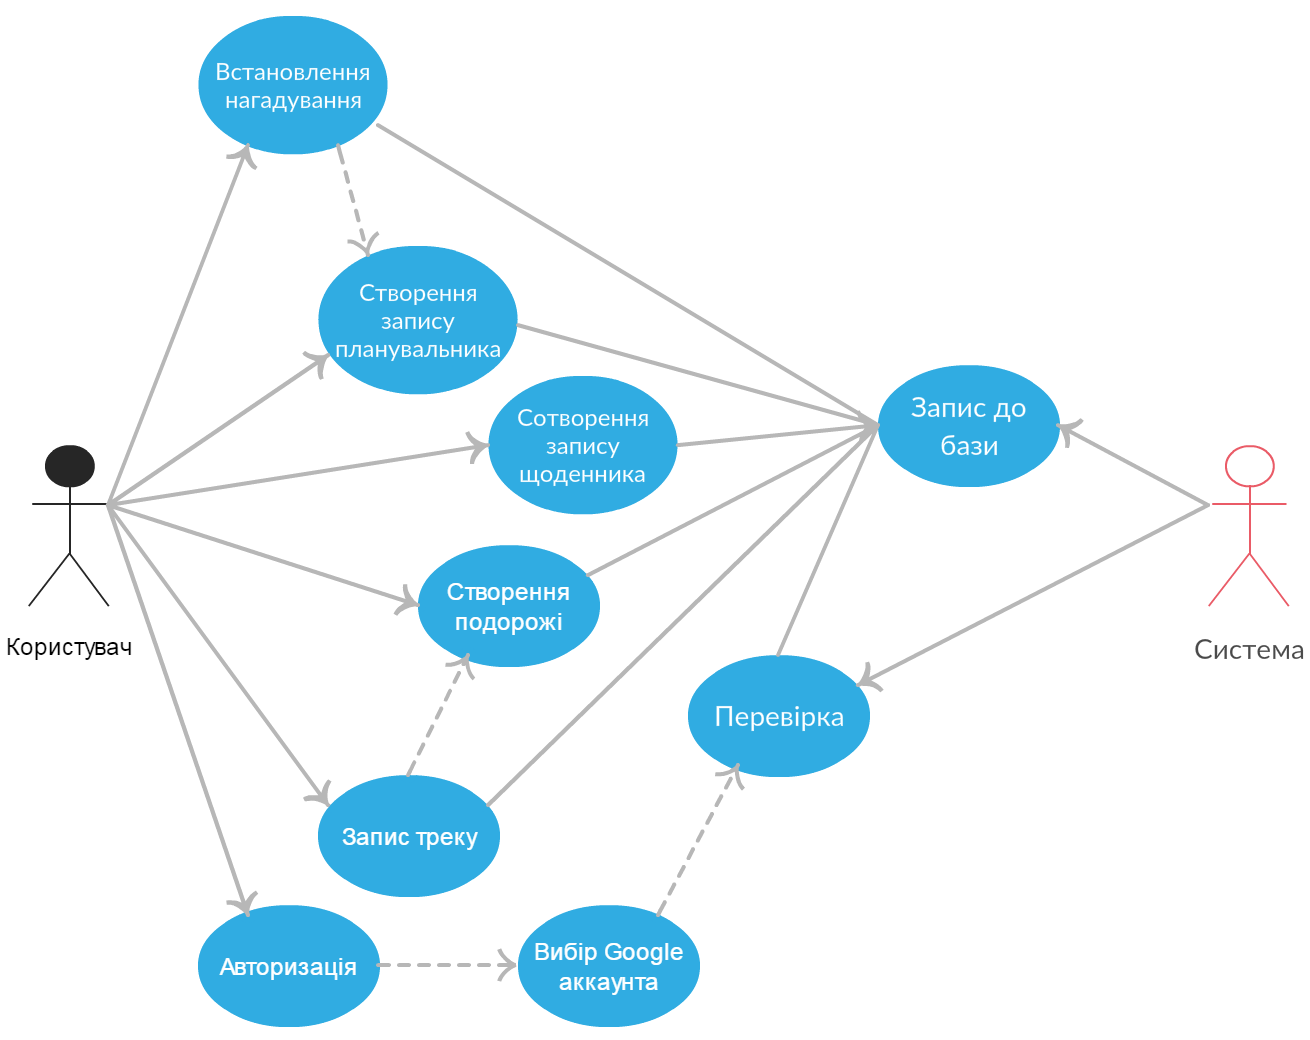
\includegraphics[width=1\textwidth]{diagram_usecase}
	\caption{Механізм роботи з додатком у вигляді діаграми прецедентів}
	\label{diagram:usecase}
\end{figure}

% TODO а воно точно нормальний вигляд має на папері? Такі ігри з кольорами часто потім мають препаршивий вигляд на папері, та й взагалі не~рекомендується перевантажувати дипломну хитрими форматуваннями

% TODO хоч я і паршиво для керівника дипломної роботи знаю ці діаграми, але факт, що акторами повинні бути лише зовнішні щодо розроблюваної системи чинники я все-таки знаю точно. До такого ТОЧНО ПРИЧЕПЛЯТЬСЯ. Якщо точно-точно нема користувачів з різними правами доступу щоб робити їх різними акторами, то, мабуть, треба зробити іншими акторами звернення до сторонніх систем... Хоча це краще ще десь уточнити.


\subsection{Формулювання та аналіз вимог за допомогою діаграми діяльності}
На основі первинних вимог були розроблені наступні детальні вимоги:
\begin{enumerate}
	\item Надати можливість редагувати подорож.
	\item Надати можливість видаляти подорож.
	\item Надати можливість редагувати запис щоденника.
	\item Надати можливість видаляти запис щоденника.
	\item Надати можливість редагувати запис планувальника.
	\item Надати можливість видаляти запис планувальника.
	\item Надати можливість додавати зображення до запису щоденника.
	\item Надати можливість переглядати карту з треком і мітками.
	\item Надати можливість обирати подорож для запису щоденника та планувальника.
	\item Надати можливість встановлювати активну подорож.
	\item Надати можливість синхронізувати дані між пристроями.
	\item Надати можливість ділитися записами щоденника через інші додатки.
	\item Надати можливість ділитися окремими зображеннями з запису щоденника через інші додатки.
	\item Надати можливість додавати списки з прапорцями в запис планувальника.
	\item Надати можливість системі автоматично завантажувати дані про погодні умови та місцезнаходження при створенні запису щоденника.
\end{enumerate}

Моделюючи поведінку системи, яка проектується або проводиться її аналіз, постає необхідність деталізувати особливості алгоритмічної і логічної реалізації виконуваних системою операцій. Для такого моделювання в мові UML використовуються діаграми діяльності.

У контексті мови UML діяльність (activity) є деякою сукупністю окремих обчислень, що виконуються автоматом. При цьому окремі елементарні обчислення можуть наводити до деякого результату або дії (action). На діаграмі діяльності відображається логіка або послідовність переходу від однієї діяльності до іншої, при цьому увага фіксується на результаті діяльності. Сам же результат може привести до зміни стану системи або повернення деякого значення.

Діаграма діяльності створення нового запису щоденника, що відображає поведінку проектованого додатка, подана на рис. \ref{diagram:activity}.

\begin{figure}[H]
	\centering
	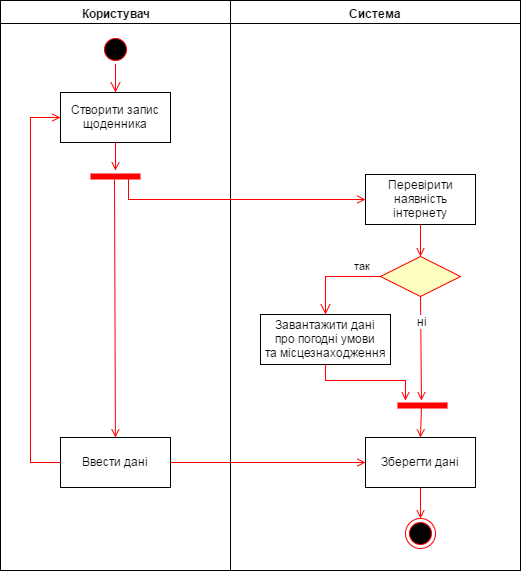
\includegraphics[width=1\textwidth]{diagram_activity}
	\caption{Механізм створення запису щоденника у вигляді діаграми діяльності}
	\label{diagram:activity}
\end{figure}

В процес створення запису щоденника залучений як користувач, так і система. Після того, як користувач вирішує створити новий запис, система, при наявності інтернет з'єднання, завантажує дані про місцезнаходження користувача на момент створення запису та дані про погодні умови в цьому місці. Після введення користувачем потрібних йому даних, та завершення створення запису, дані зберігаються.

\subsection{Аналіз вимог за допомогою діаграми послідовності}
На базі отриманих даних, і заради детальнішого моделювання була розроблена діаграма послідовностей для процесу сотворення запису планувальника та встановлення нагадування.

На діаграмі послідовності об’єкт зображується у вигляді прямокутника на вершині пунктирної вертикальної лінії. Ця вертикальна лінія називається лінією життя об’єкту. Вона є фрагментом життєвого циклу об’єкту в процесі взаємодії. Кожне повідомлення представляється у вигляді стрілки між лініями життя двох об’єктів. Повідомлення з’являються в тому порядку, як вони показані на діаграмі (зверху вниз). Кожне повідомлення може бути позначене ім’ям.

Як видно з діаграми послідовності (див. рис. \ref{diagram:sequence}), після створення нагадування, дані записуються до бази даних та відбувається встановлення будильників у системі. 

\begin{figure}[H]
	\centering
	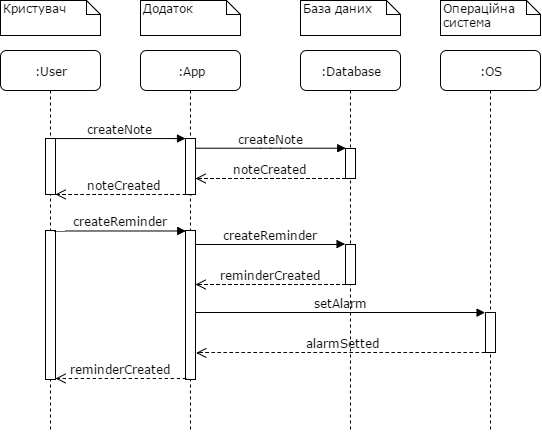
\includegraphics[width=0.85\textwidth]{diagram_sequence}
	\caption{Діаграма послідовності створення запису планувальника та встановлення нагадування}
	\label{diagram:sequence}
\end{figure}

\subsection{Аналіз вимог за допомогою діаграми комунікації}
Діаграми комунікації відображають взаємодію ролей або об'єктів у процесі функціонування системи, описують обмін даними (повідомленнями) між різними учасниками взаємодії. Такі діаграми моделюють сценарії поведінки системи \cite{diploma_guidelines}. 

Діаграма комунікації для процесу перегляду подорожі та створення запису щоденника зображена на рис. \ref{diagram:communication}.

\begin{figure}[H]
	\centering
	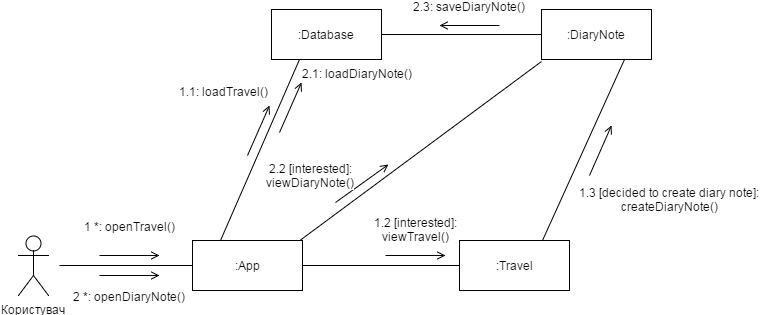
\includegraphics[width=1\textwidth]{diagram_communication}
	\caption{Механізм перегляду подорожей та записів щоденника у вигляді діаграми комунікації}
	\label{diagram:communication}
\end{figure}

При виборі користувачем подорожі чи запису щоденника, дані завантажуються з бази даних, та відображаються користувачеві. Також, знаходячись на екрані перегляду подорожі, користувач може вирішити створити запис щоденника для цієї подорожі.

\section{Визначення поведінки об'єктів системи}

%TODO

\section{Висновки}

% TODO: Висновки обсягом 0,5-1 с.

\end{document}
